%-----------------------------------LICENSE------------------------------------%
%   This file is part of Mathematics-and-Physics.                              %
%                                                                              %
%   Mathematics-and-Physics is free software: you can redistribute it and/or   %
%   modify it under the terms of the GNU General Public License as             %
%   published by the Free Software Foundation, either version 3 of the         %
%   License, or (at your option) any later version.                            %
%                                                                              %
%   Mathematics-and-Physics is distributed in the hope that it will be useful, %
%   but WITHOUT ANY WARRANTY; without even the implied warranty of             %
%   MERCHANTABILITY or FITNESS FOR A PARTICULAR PURPOSE.  See the              %
%   GNU General Public License for more details.                               %
%                                                                              %
%   You should have received a copy of the GNU General Public License along    %
%   with Mathematics-and-Physics.  If not, see <https://www.gnu.org/licenses/>.%
%------------------------------------------------------------------------------%
%       Author: Ryan Maguire                                                   %
%       Date:   2023/10/14                                                     %
%------------------------------------------------------------------------------%
\documentclass{article}
\usepackage[margin=1in]{geometry}
\usepackage{amssymb}
\usepackage{amsmath}
\usepackage{graphics}
\usepackage{hyperref}
\hypersetup{colorlinks=true, linkcolor=blue}
\title{Teaching Statement}
\author{Ryan Maguire}
\date{\today}
\begin{document}
    \maketitle
    In the U.S. many students are (erroneously) convinced that
    mathematics is a game of memorization, using the correct formula in the
    correct place to get the correct answer. They then tend to \textit{hate}
    mathematics with a passion. This is not entirely their fault. To paraphrase
    Edward Frenkel,
    \textit{Would you love art if you were only taught how to paint a fence}?
    It then becomes the job of the mathematics educator to convince their
    students that mathematics is not \textit{painting a fence}, but rather
    a collection of \textit{works of art}.
    \par\hfill\par
    In many instances this can be a surprisingly easy task, you simply need to
    have the right \textit{painting} at hand.
    A pre-calculus student who knows about complex
    numbers (usually taught in U.S. high schools) and function compositions
    (taught in a pre-calculus course) has all of the tools needed to understand
    the construction of the beautiful Glynn fractal, a variant of the
    Mandelbrot set (see Fig.~\ref{fig:glynn_fractal}).%
    \footnote{%
        The source code for this figure is free software:
        \url{https://github.com/ryanmaguire/libtmpl/}
    }
    Students of calculus are often taught Newton's method towards the end
    of the semester, but are almost always denied the beauty of Newton basins
    (Fig.~\ref{fig:newton_fractal}).%
    \footnote{%
        Similarly for this figure:
        \url{https://github.com/ryanmaguire/newton_fractals/}
    }
    Almost every branch of mathematics has a beautiful painting associated with
    it, you simply need to draw it.
    \par\hfill\par
    With these two examples in mind
    it may come as no surprise that I am a big fan of mathematical
    visualization. For me, being able to \textit{see} a concept helps it settle
    in far greater than doing exercises or seeing examples (those these are
    important too). To this end I've attempted to contribute to the
    visualization community by created figures of my own. I have written
    code for 520+ figures in \texttt{asymptote}, 130+ in \texttt{tikz},
    50+ in \texttt{C} (including the three figures below), and a handful in
    \texttt{POV-Ray}. All of this I make available as free software.%
    \footnote{%
        See
        \url{https://github.com/ryanmaguire/Mathematics-and-Physics/}
    }
    \par\hfill\par
    Finding the right painting can be highly dependent on the scenario the
    mathematics instructor finds themselves in. In the summer of 2022 I had the
    pleasure of teaching my favorite course, point-set topology, at Dartmouth
    college. There were a handful of students (16 on the roster, plus a few
    auditors), and the course was progressing in a rather standard manner
    (set theory, topological spaces, metric spaces, and so on). At the
    end of the class I always say \textit{Okay, toodles!} as an informal
    farewell to the students. Several of my Chinese students approached me at
    the end of class one day and asked me
    \textit{Why do you keep calling us potatoes}?
    It was then that I learned \textit{tu-dou} means potato in Chinese, similar
    enough to cause the confusion. I used this as an opportunity to discuss
    \textit{perfectly normal topological spaces}.
    Given a metric space $(X,\,d)$ we can separate any two disjoint closed
    subsets $\mathcal{C}$ and $\mathcal{D}$ via:
    \begin{equation}
        f(x)=
        \frac{\textrm{dist}(x,\,\mathcal{C})}
             {\textrm{dist}(x,\,\mathcal{C})+\textrm{dist}(x,\,\mathcal{D})}
    \end{equation}
    Since Euclidean spaces are metric spaces
    (with the standard Euclidean metric) we can make this far more concrete if
    we use the Euclidean plane as our motivating example. Given any closed
    regions $\mathcal{C}$ and $\mathcal{D}$ that are themselves the finite
    union of closed polygonal figures, it becomes a straight-forward
    calculation to compute
    $\textrm{dist}\big((x,\,y),\,\mathcal{C}\big)$ and
    $\textrm{dist}\big((x,\,y),\,\mathcal{D}\big)$, respectively, for any point
    $(x,\,y)$ in the plane. We can then compute $f$ directly. Since the image
    of the function is $[0,\,1]$, to each point in the plane we can associate
    a color which varies smoothly between red and blue depending on the value of
    $f$ at that point. That is, 0 maps to red, 1 to blue, and a continuous
    rainbow gradient for values in between. We can construct the Chinese
    characters for \textit{tu-dou} using polygons, and with all this in mind
    the concept of \textit{perfectly normal topological spaces} becomes quite
    visual (see Fig.~\ref{fig:potato}).
    \footnote{%
        Source code for this is available:
        \url{https://github.com/ryanmaguire/perfectly_normal_spaces/}
    }
    \begin{figure}
        \centering
        \resizebox{\textwidth}{!}{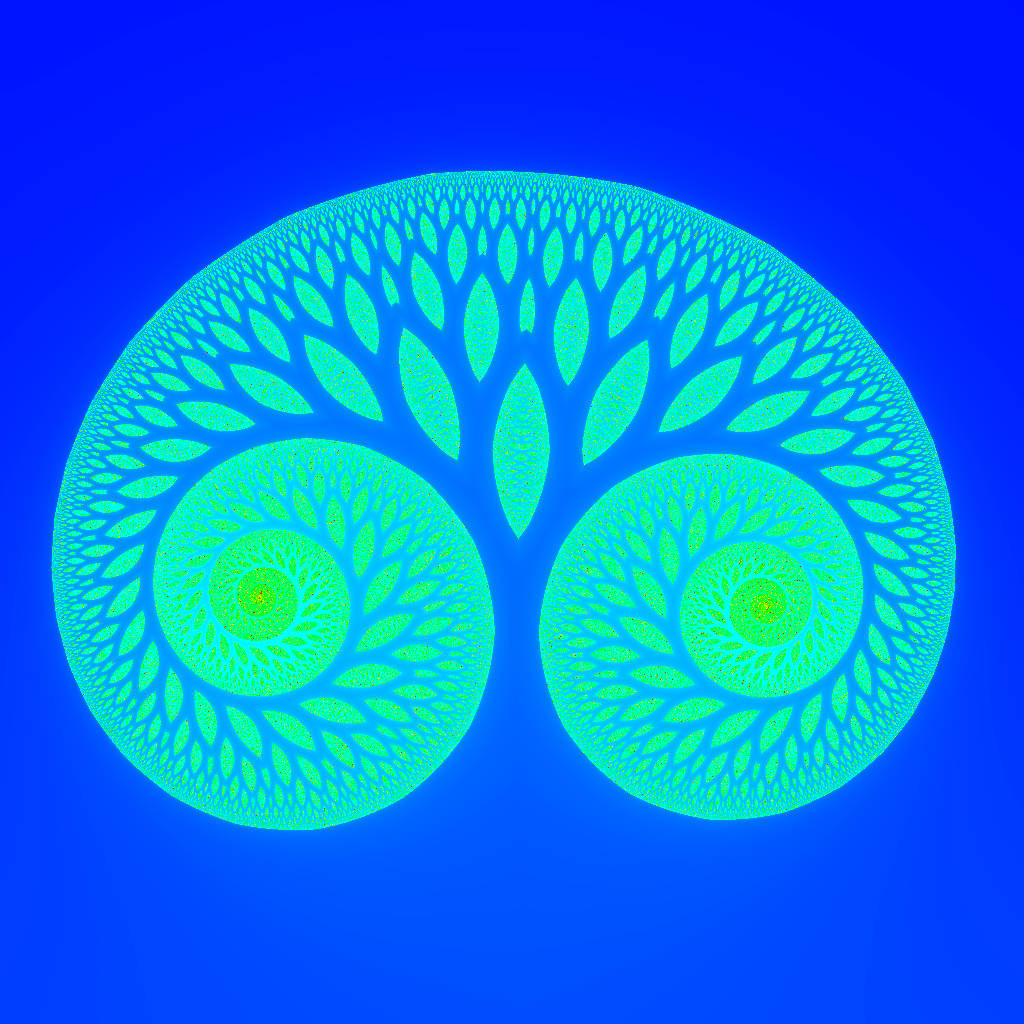
\includegraphics{glynn_fractal.png}}
        \caption{The Glynn Fractal}
        \label{fig:glynn_fractal}
    \end{figure}
    \begin{figure}
        \centering
        \resizebox{\textwidth}{!}{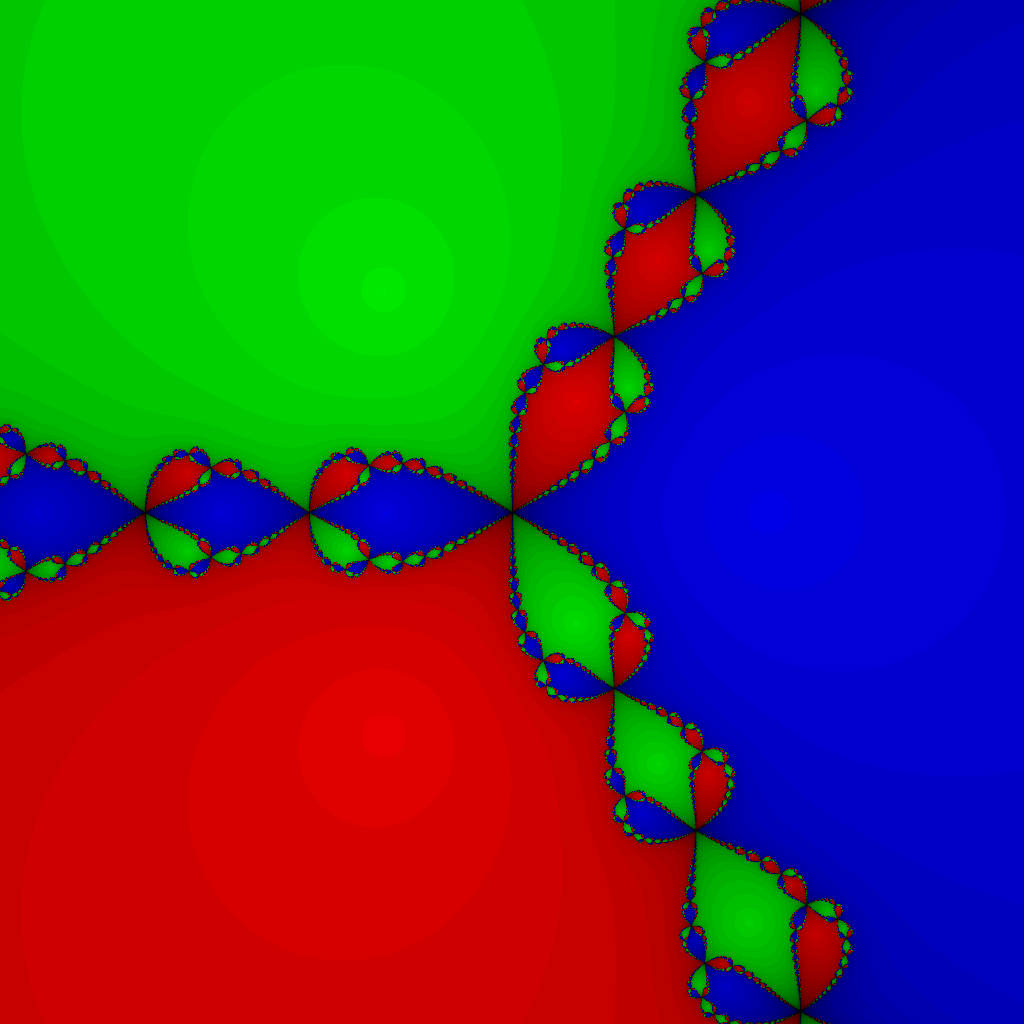
\includegraphics{newton_fractal.png}}
        \caption{The Newton Fractal}
        \label{fig:newton_fractal}
    \end{figure}
    \begin{figure}
        \centering
        \resizebox{\textwidth}{!}{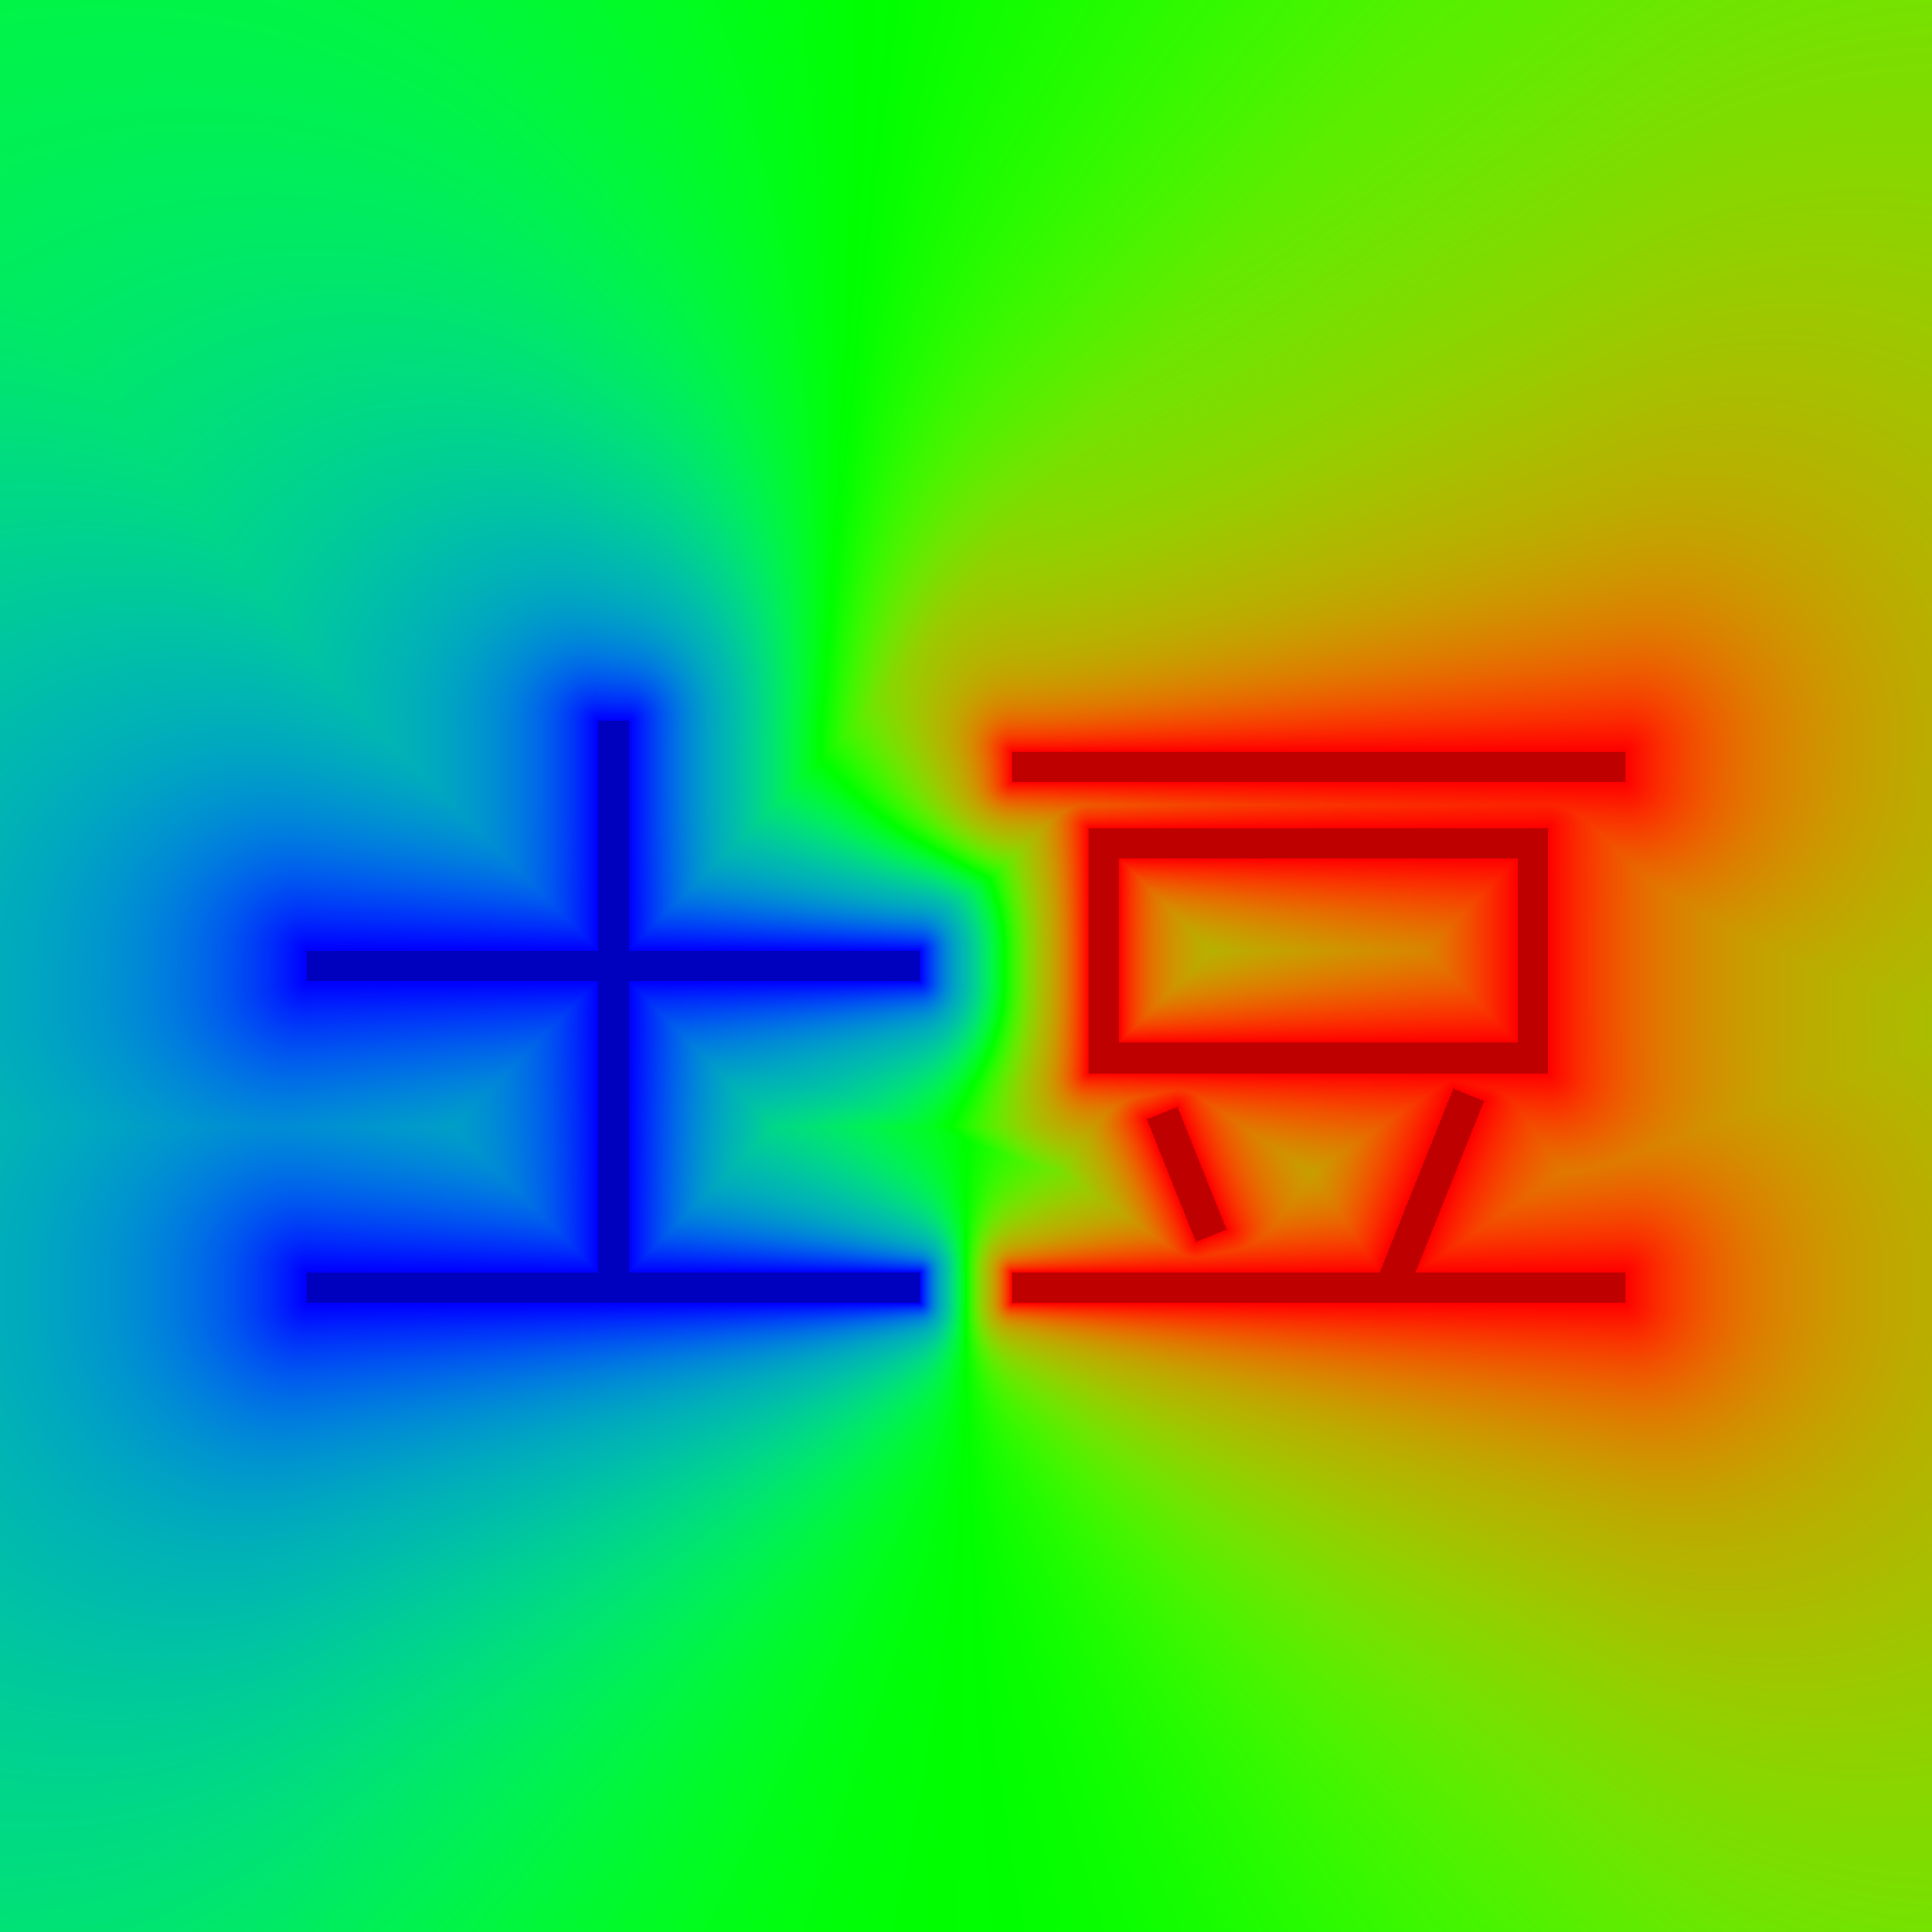
\includegraphics{potato.png}}
        \caption{Perfectly Normal Topological Spaces}
        \label{fig:potato}
    \end{figure}
\end{document}
